%seminarska naloga
\documentclass[seminar, slovene]{FRIreport}

% AMS fonts required
\usepackage{iopams}  

% package to include graphics in ps, eps or png format
\usepackage{graphicx}
\usepackage{epstopdf}
% the graphics path
\graphicspath{{img/}}

\usepackage{float}

% define equation referencing
\newcommand{\eqref}[1]{(\ref{#1})}

% define figure referencing
\newcommand{\figref}[1]{\ref{#1}}

% define real numbers symbol
\newcommand{\Rset}{\ensuremath{\mathbb{R}}} 
\newcommand{\R}{\Rset} 
% define natural numbers symbol
\newcommand{\Nset}{\ensuremath{\mathbb{N}}} 
\newcommand{\N}{\Nset} 
% define euclidean vector space symbol
\newcommand{\Eset}{\ensuremath{\mathbb{E}}} 
\newcommand{\E}{\Eset} 

\newcommand{\imp}[1]{{\color{P654M}#1\normalcolor}}

%%%
\newcommand{\angl}[1]{(\textit{angl.} #1)}

\setcounter{tocdepth}{2}

%main
\begin{document}

\title{QCA sekven\v cna ALE}

\author{Miha Zidar, Anže Pečar, Matic Potočnik, Željko Plesac, Jan Varljen}

\address{Skupina 2 in 4}

\begin{abstract}
V seminarski nalogi bomo opisali zasnovo sekvenčne ALE s kvantnimi celičnimi avtomati, z uporabo programa QCAdesigner.

\Keywords{kvantni celični avtomati, aritmetično-logična enota, modeliranje in simulacija}
\end{abstract}

%
%%
\section{Uvod}
\subsection{Ideja}
V tej seminarski nalogi bomo opisali realizacijo sekvenčne ALE s kvantnimi celičnimi avtomati \angl{quantum cellular automata -- QCA}. Modelirali jo bomo z uporabo odprtokodnega programa QCADesigner\cite{walus:2004}, za skice logičnih vezij, pa bomo uporabili (tudi odprtokoden) program TinyCAD.
\ \\ \ \\
Sekvenčnost enote v tem kontekstu pomeni, da enota ne izvaja operacij nad vsebino končno dolgih registrov, kot smo navajeni pri klasični ALE, ampak sprejema tok bitov, izvaja operacije nad posameznimi biti, ter tudi svoj izhod podaja kot tok bitov. Za določene operacije tak pristop ni praktičen, ali pa je celo nemogoč (Primer: deljenje, korenjenje, kotne funkcije). Je pa na tak način mogoče implementirati poln funkcijski sistem, kar je cilj te seminarske naloge.

\subsection{Motivacija}
Predvideva se, da bo že čez nekaj desetletij minituarizacija in zmogljivost čipov, grajenih na siliciju, dosegla končno stopnjo in bo potrebno za večjo procesno moč preiti na drug osnovni material in najverjetneje tudi precej spremeniti pristop k modeliranju vezij. Ena izmed obetajočih alternativ so kvantni celični avtomati, ki obljubljajo mnoge prednosti pred klasičinimi vezji:
\begin{itemize}
\item Možnost večnivojskih vezij
\item Možnost križanja vodil
\item Enostavna realizacija nekaterih časovnih vezij
\item Potencialno nižja poraba in višji takt delovanja
\item $\dots$
\end{itemize}
\pagebreak
%
%%
\section{Metode}
V tem odseku bomo predstavili nekatere osnovne ideje in odločitve, ki smo jih nato uporabili pri realizaciji naše ALE.

\subsection{Osnovni opis enote}
Realizirali bomo sekvenčno ALE, s funkcijsko polnim funkcijskim sistemom operacij. Enota bo imela dva podatkovna vhoda, ter dva vhoda za izbiro operacije. Enota bo podpirala naslednje operacije:\\
\begin{table}[H]
\begin{center}
\begin{tabular}{ | c | c | c | }\hline
\textbf{Operacija} & \textbf{Oznaka} & \textbf{Op. koda} \\ \hline
Negacija & NOT & 0\,0 \\
Konjunkcija & AND & 0\,1 \\
Seštevanje & ADD & 1\,0 \\
Odštevanje & SUB & 1\,1 \\ \hline
\end{tabular}
\caption{Seznam operacij}
\label{optable}
\end{center}
\end{table}
\subsection{Ideje za realizacijo}
\subsubsection{Glede sekvenčnosti}\ \\ \ \\
Operaciji NOT in AND sta že v osnovi bitni operaciji in je tako sekvenčna realizacija popolnoma naravna. Pri ADD s stališča sekvenčnosti delovanja tudi ni posebnih zapletov, pri SUB pa lahko poskušamo operirati, kot bi imeli števili zapisani v predstavitvi z dvojnim komplementom.

\subsubsection{Modeliranje}\ \\ \ \\
Za modeliranje bomo, kot že omenjeno, uporabili program QCAdesigner.
\begin{figure}[H]
\begin{center}
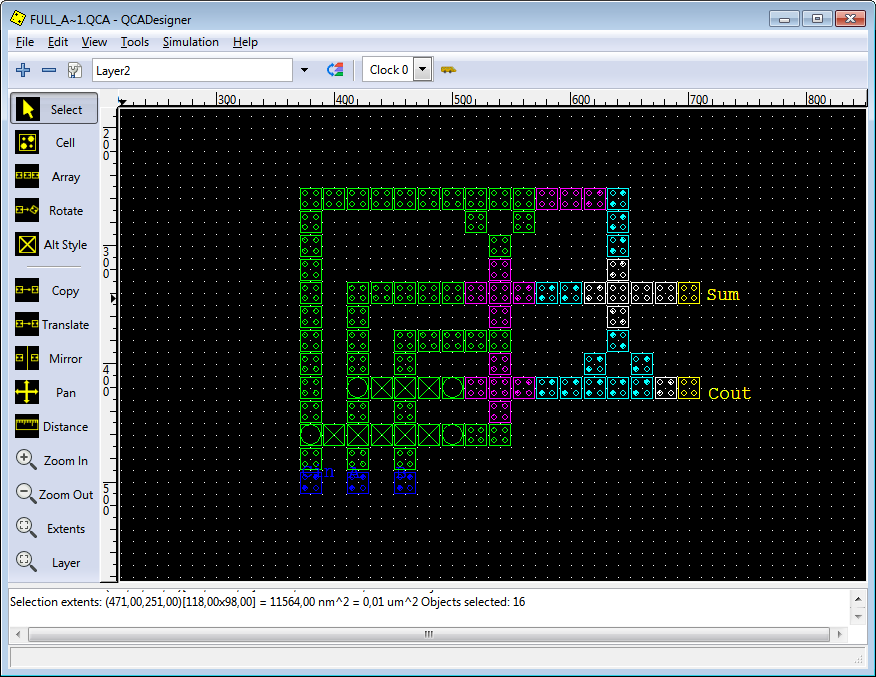
\includegraphics[width=8.65cm]{qca/img/qcadesigner}
\caption{QCAdesigner}
\end{center}
\end{figure}
%
%%
\section{Rezultati}
V tem delu seminarske naloge bomo predstavili realizacijo posameznih delov ALE. Pri realizaciji smo si pomagali s knjigo\cite{virant:2007}, ter diplomsko nalogo\cite{orac:2007}.
\subsection{Shema enote}
Imamo podatkovni liniji $X_1$ in $X_2$, ter naslovni liniji $A_1$ in $A_2$, ter izhod $Y$. Najprej z $A_1$ izberemo seštevanje(ADD) oz. odštevanje(SUB), ki sta realizirani v eni enoti. Operaciji konjunkcija(AND) in negacija(NOT) se vedno izvedeta, nato pa na koncu še izberemo, kateri izmed izhodov operacij se bo pojavil na izhodu $Y$.
\begin{figure}[H]
\begin{center}
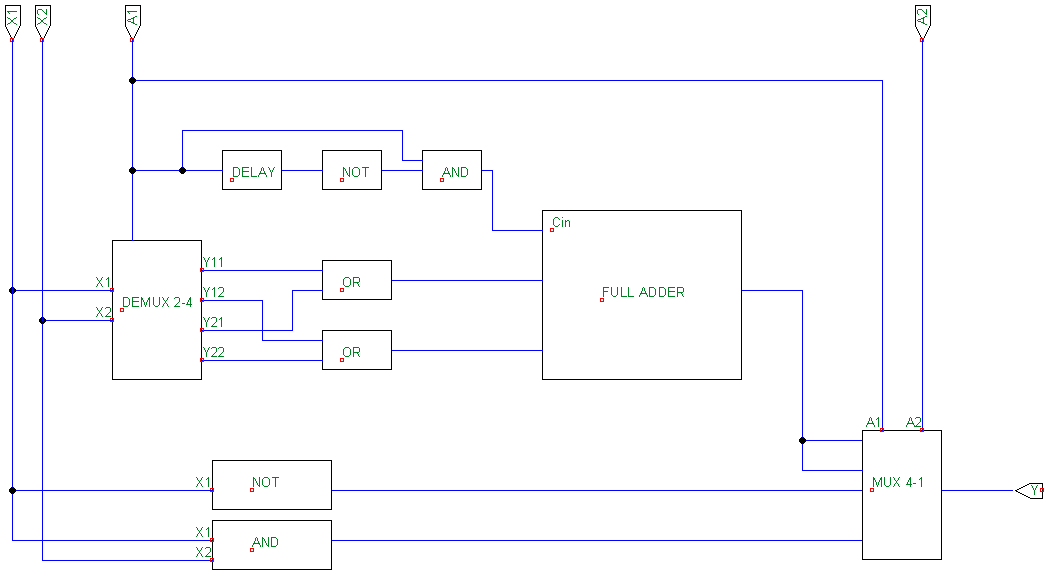
\includegraphics[width=16cm]{vezja/img/alu}
\caption{Shema celotne enote}
\end{center}
\end{figure}

\begin{minipage}[H]{16cm}
\subsection{Izbira operacije}
Izbira med ADD in SUB:\\
\begin{figure}[H]
\begin{center}
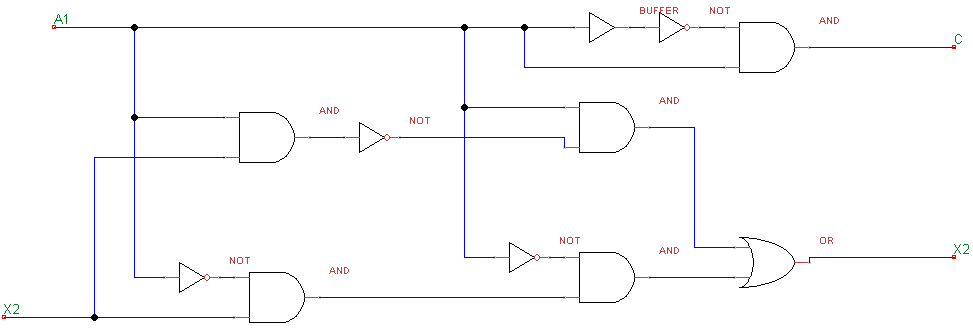
\includegraphics[width=13cm]{vezja/img/demuxmux}
\end{center}
\end{figure}
\begin{figure}[H]
\begin{center}
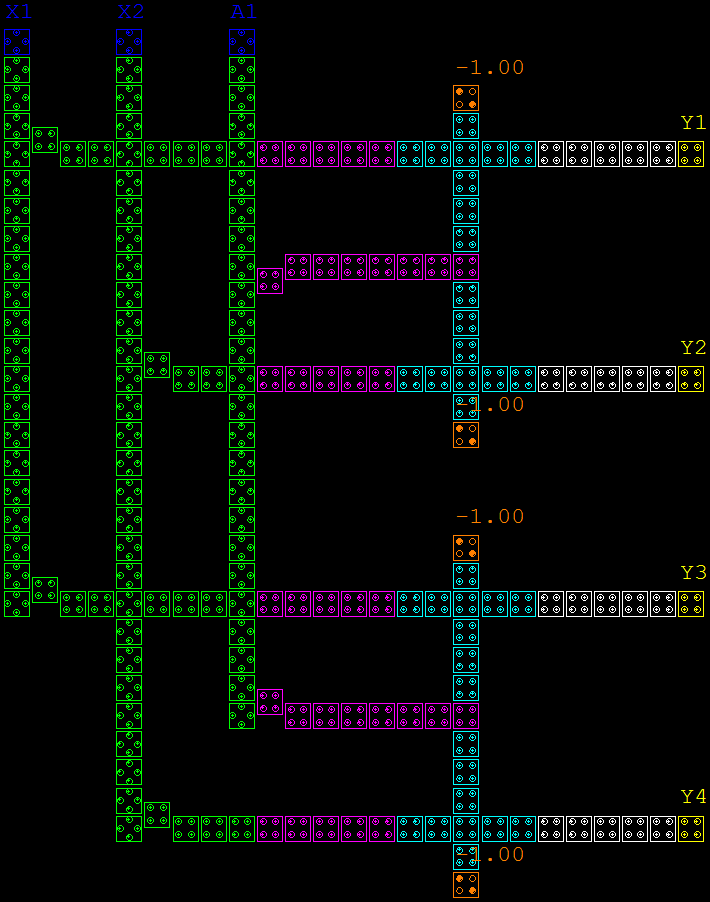
\includegraphics[width=13cm]{qca/img/demuxmux}
\end{center}
\end{figure}
\end{minipage}

\begin{minipage}[H]{16cm}
Izbira rezultata:\\
\begin{center}
\begin{figure}[H]
\begin{center}
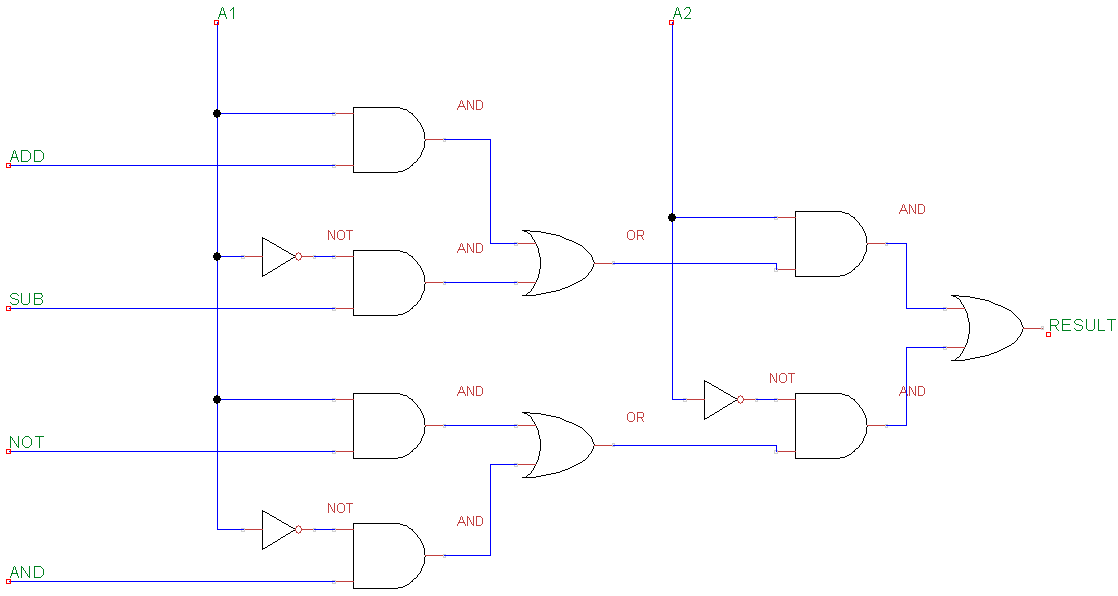
\includegraphics[width=12cm]{vezja/img/mux}
\end{center}
\end{figure}
\begin{figure}[H]
\begin{center}
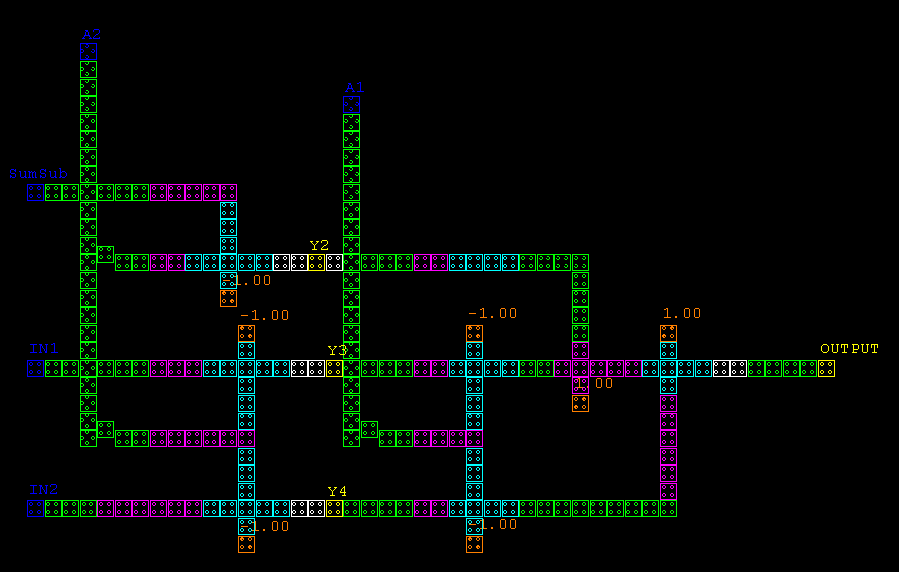
\includegraphics[width=13cm]{qca/img/mux}
\end{center}
\end{figure}
\end{center}
\end{minipage}

\subsection{Negacija (NOT)}
\subsubsection{Opis operacije}\ \\ \ \\
Negacija vrne obratno vrednost vhoda -- torej za 0 vrne 1 in obratno.
\ \\
\begin{table}[H]
\begin{center}
Enačba: $ Y = \lnot X_1 $\\  \ \\
\begin{tabular}{ | c || c | }\hline
$X_1$ & $Y$ \\ \hline
0 & 1 \\
1 & 0 \\ \hline
\end{tabular}\\ \ \\ \ \\
Pravilnostna tabela NOT
\end{center}
\end{table}

\subsubsection{Realizacija}\ \\ \ \\
Negacijo smo realizirali s polovičnim zamikom QCA celic.
\begin{figure}[H]
\begin{center}
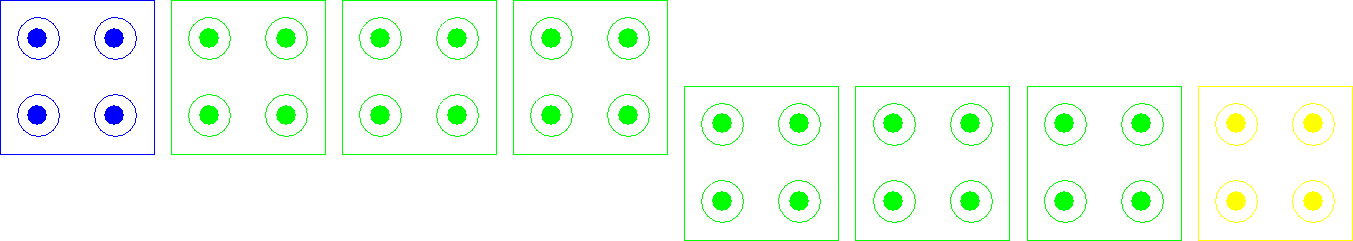
\includegraphics[width=8cm]{qca/img/NOT}
\caption{NOT vrata}
\label{NOT}
\end{center}
\end{figure}
\subsection{Konjunkcija (AND)}
\subsubsection{Opis operacije}\ \\ \ \\
Konjunkcija vrne 1 natanko takrat, kadar imata oba vhoda vrednost 1.
\ \\
\begin{table}[H]
\begin{center}
Enačba: $ Y = X_1 \wedge X_2 $\\ \ \\
\begin{tabular}{ | c | c || c | }\hline
$X_1$ & $X_2$ & $Y$ \\ \hline
0 & 0 & 0\\
0 & 1 & 0\\
1 & 0 & 0\\
1 & 1 & 1\\ \hline
\end{tabular}\\ \ \\ \ \\
Pravilnostna tabela AND
\end{center}
\end{table}

\subsubsection{Realizacija}\ \\ \ \\
Konjunkcijo smo realizirali z majoritetnimi vrati, ki imajo enega izmed vhodov nastavljenega na polarizacijo -1.
\begin{figure}[H]
\begin{center}
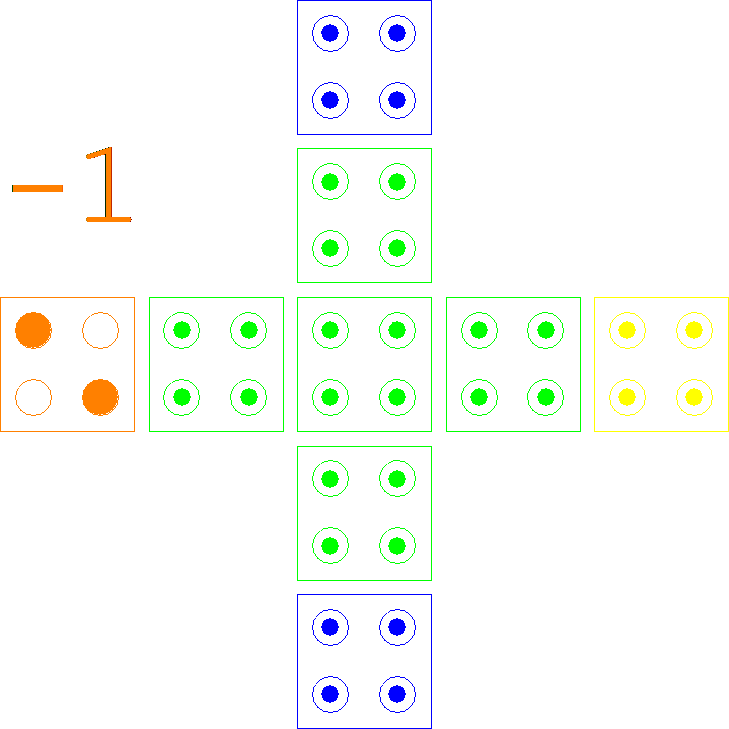
\includegraphics[width=5cm]{qca/img/AND}
\caption{AND vrata}
\label{AND}
\end{center}
\end{figure}

\subsection{Seštevalnik(ADD) / Odštevalnik(SUB)}
\subsubsection{Opis operacije}\ \\ \ \\
Seštevalnik izvede seštevanje vhodov $X_1$, $X_2$ in prenosa $C$. Izhoda sta vsota vseh treh vhodov, ter prenos, ki se v naši enoti prenese nazaj kot prenos $C$ za naslednje seštevanje.
\ \\
\begin{table}[H]
\begin{center}
Enačba:\\
$Y = (X_1 \oplus X_2) \oplus C$\\
$C_{out} = (X_1 \wedge X_2) \vee (C \wedge X_2) \vee (C \wedge X_1) $\\ \ \\
\begin{tabular}{ | c | c | c || c | c | }\hline
$X_1$ & $X_2$ & $C$ & $Y$ & $c_{out}$ \\ \hline
0 & 0 & 0 & 0 & 0\\
0 & 0 & 1 & 1 & 0\\
0 & 1 & 0 & 1 & 0\\
0 & 1 & 1 & 0 & 1\\
1 & 0 & 0 & 1 & 0\\
1 & 0 & 1 & 0 & 1\\
1 & 1 & 0 & 0 & 1\\
1 & 1 & 1 & 1 & 1\\ \hline
\end{tabular}\\ \ \\ \ \\
Pravilnostna tabela ADD
\end{center}
\end{table}
\ \\
\begin{figure}[H]
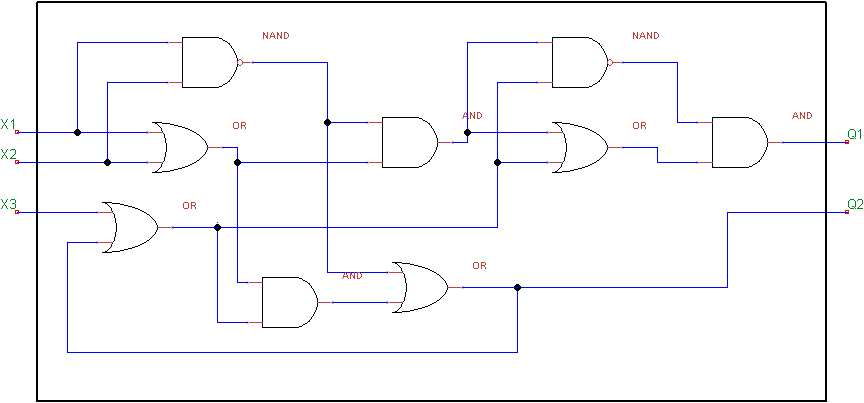
\includegraphics[width=14cm]{vezja/img/adder}
\caption{Seštevalnik}
\label{sestevalnik}
\end{figure}
\ \\
Odštevalnik deluje zelo podobno seštevalniku, le da vhode odšteje med seboj.
\ \\
\begin{table}[H]
\begin{center}
Enačba:\\
$Y = (X_1 \oplus X_2) \oplus C$\\
$C_{out} = (C \wedge (X_1 \equiv X_2)) \vee (\overline{X_1} \wedge X_2) $\\ \ \\
\begin{tabular}{ | c | c | c || c | c | }\hline
$X_1$ & $X_2$ & $C$ & $Y$ & $C_{out}$ \\ \hline
0 & 0 & 0 & 0 & 0\\
0 & 0 & 1 & 1 & 1\\
0 & 1 & 0 & 1 & 1\\
0 & 1 & 1 & 0 & 1\\
1 & 0 & 0 & 1 & 0\\
1 & 0 & 1 & 0 & 0\\
1 & 1 & 0 & 0 & 0\\
1 & 1 & 1 & 1 & 1\\ \hline
\end{tabular}\\ \ \\ \ \\
Pravilnostna tabela SUB
\end{center}
\end{table}

\subsubsection{Realizacija}\ \\ \ \\
Seštevalnik in odštevalnik (operaciji ADD in SUB), smo želeli realizirali v eni enoti. Pri tem smo se pri odštevanju obnašali, kot bi operirali v predstavitvi z dvojnim komplementom. To pomeni, da $X_2$ negiramo in ob prvem odštevanju $C$ nastavimo na 1.\\
\ \\
\begin{minipage}[H]{16cm}
Naša realizacija seštevalnika:
\begin{figure}[H]
\begin{center}
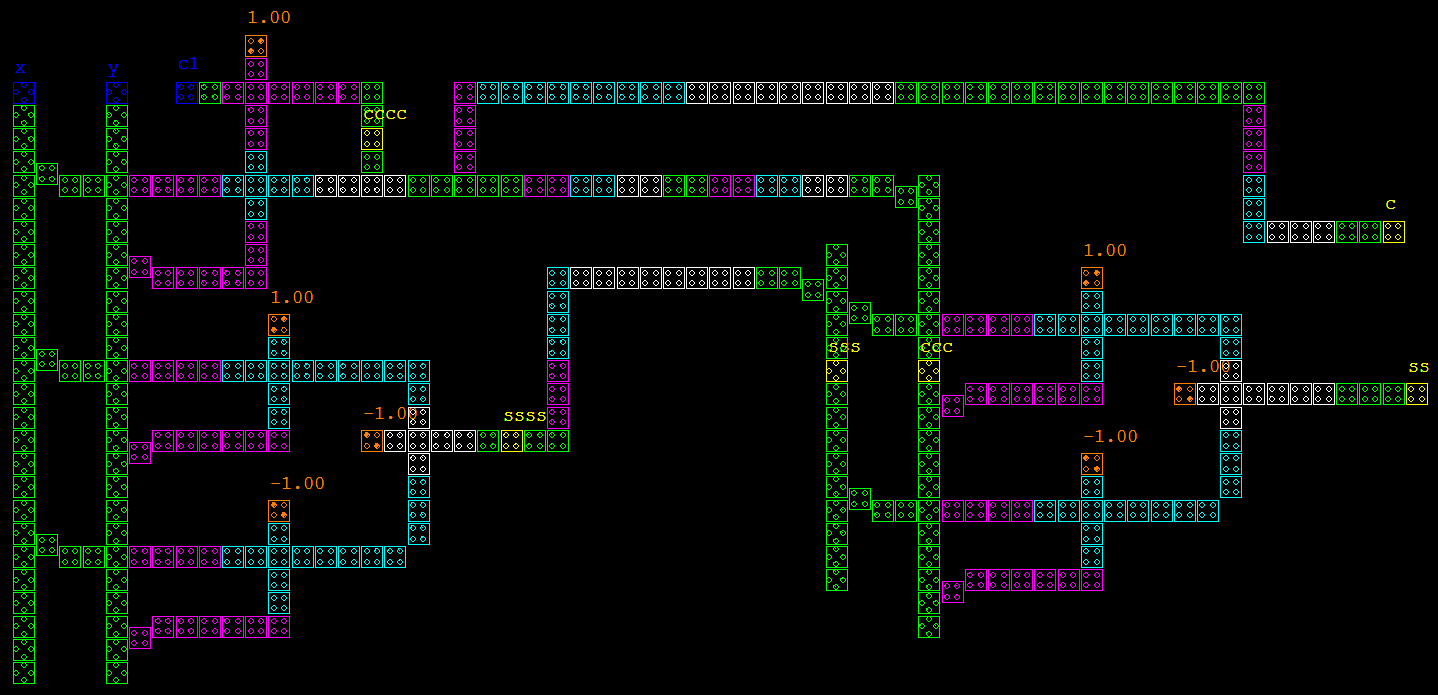
\includegraphics[width=16cm]{qca/img/sum}
\caption{Seštevalnik}
\label{sestevalnikqca}
\end{center}
\end{figure}
Prikaz delovanja seštevalnika:
\begin{figure}[H]
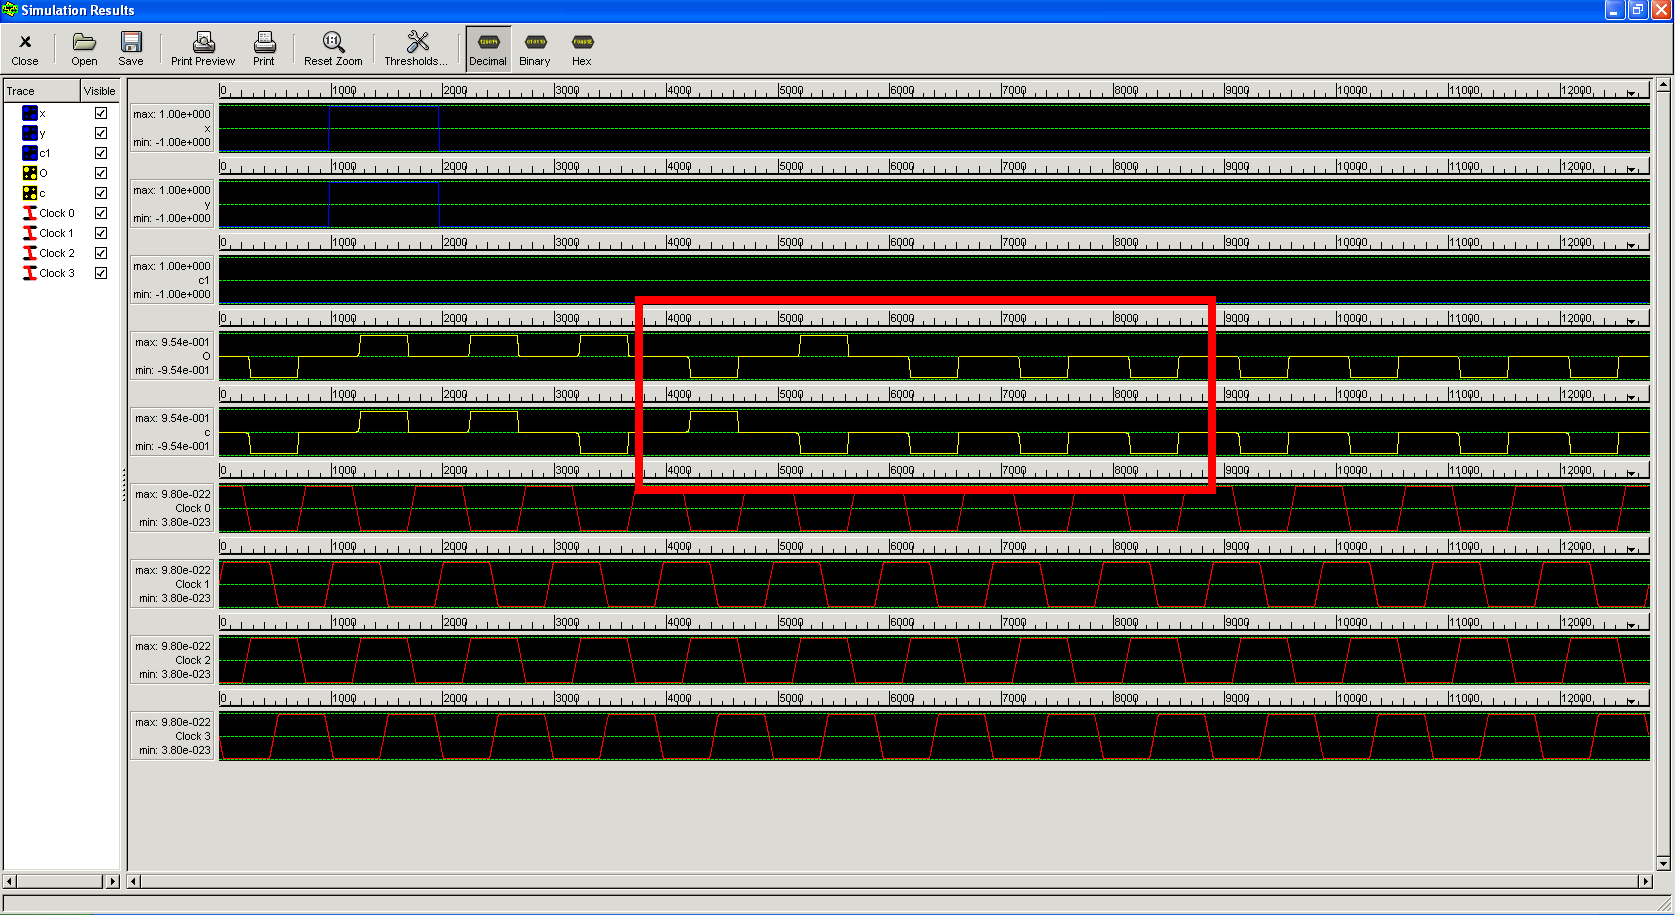
\includegraphics[width=14cm]{simulacije/1+1}
\caption{1+1=2}
\label{1+1}
\end{figure}
\end{minipage}
\begin{minipage}[H]{16cm}
\begin{figure}[H]
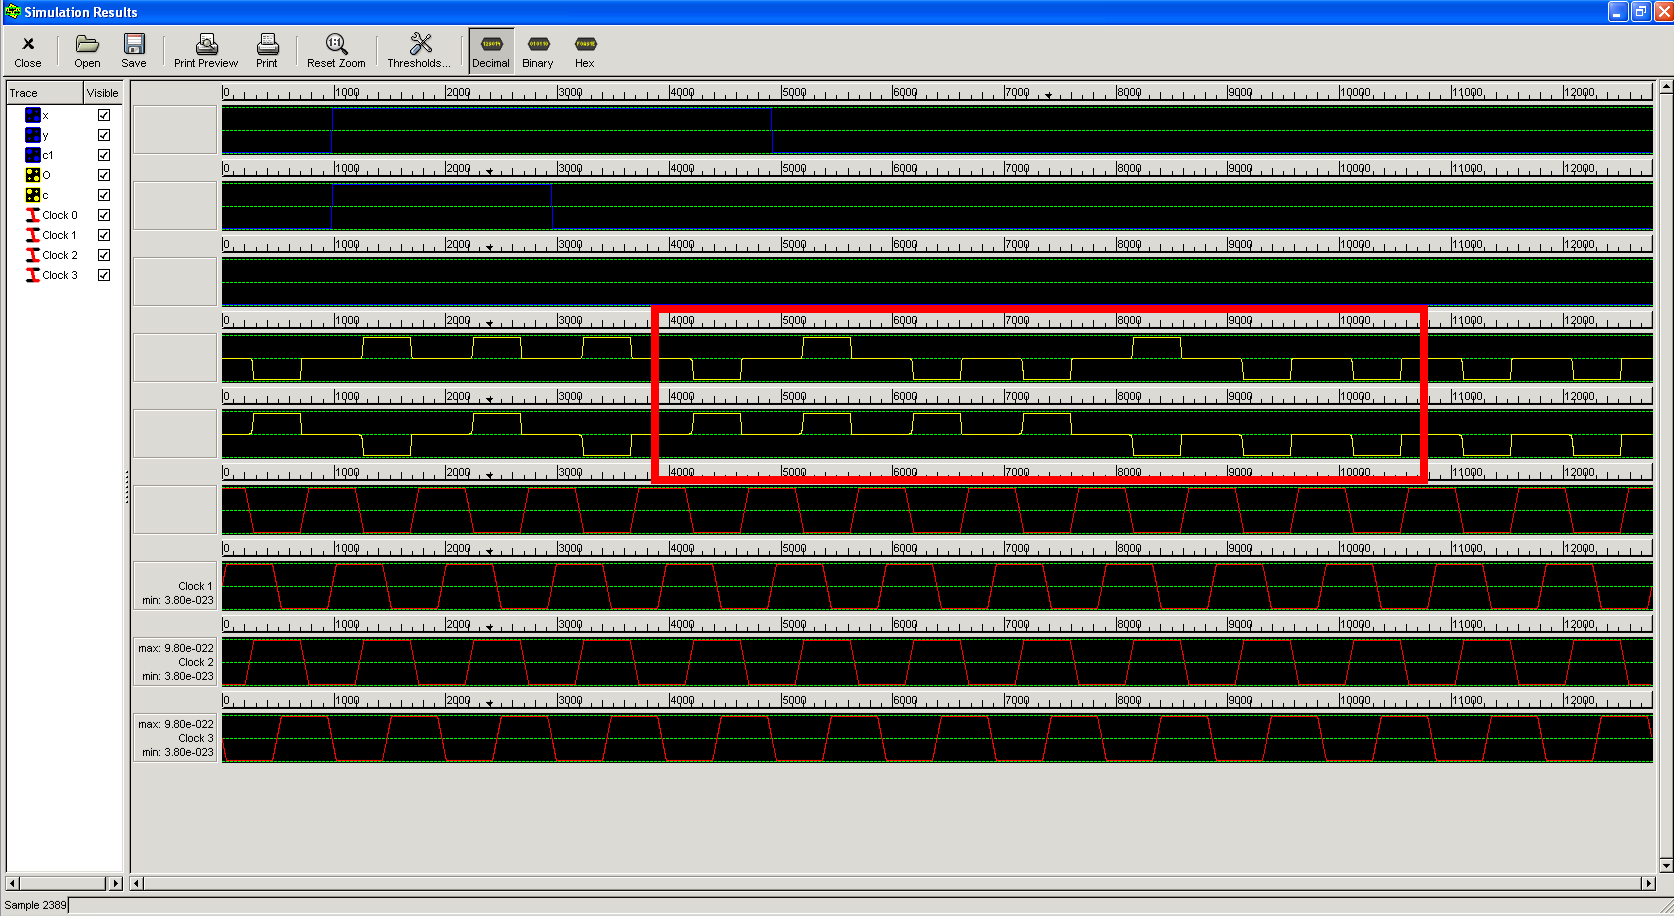
\includegraphics[width=14cm]{simulacije/3+15}
\caption{3+15=18}
\label{3+15}
\end{figure}
\begin{figure}[H]
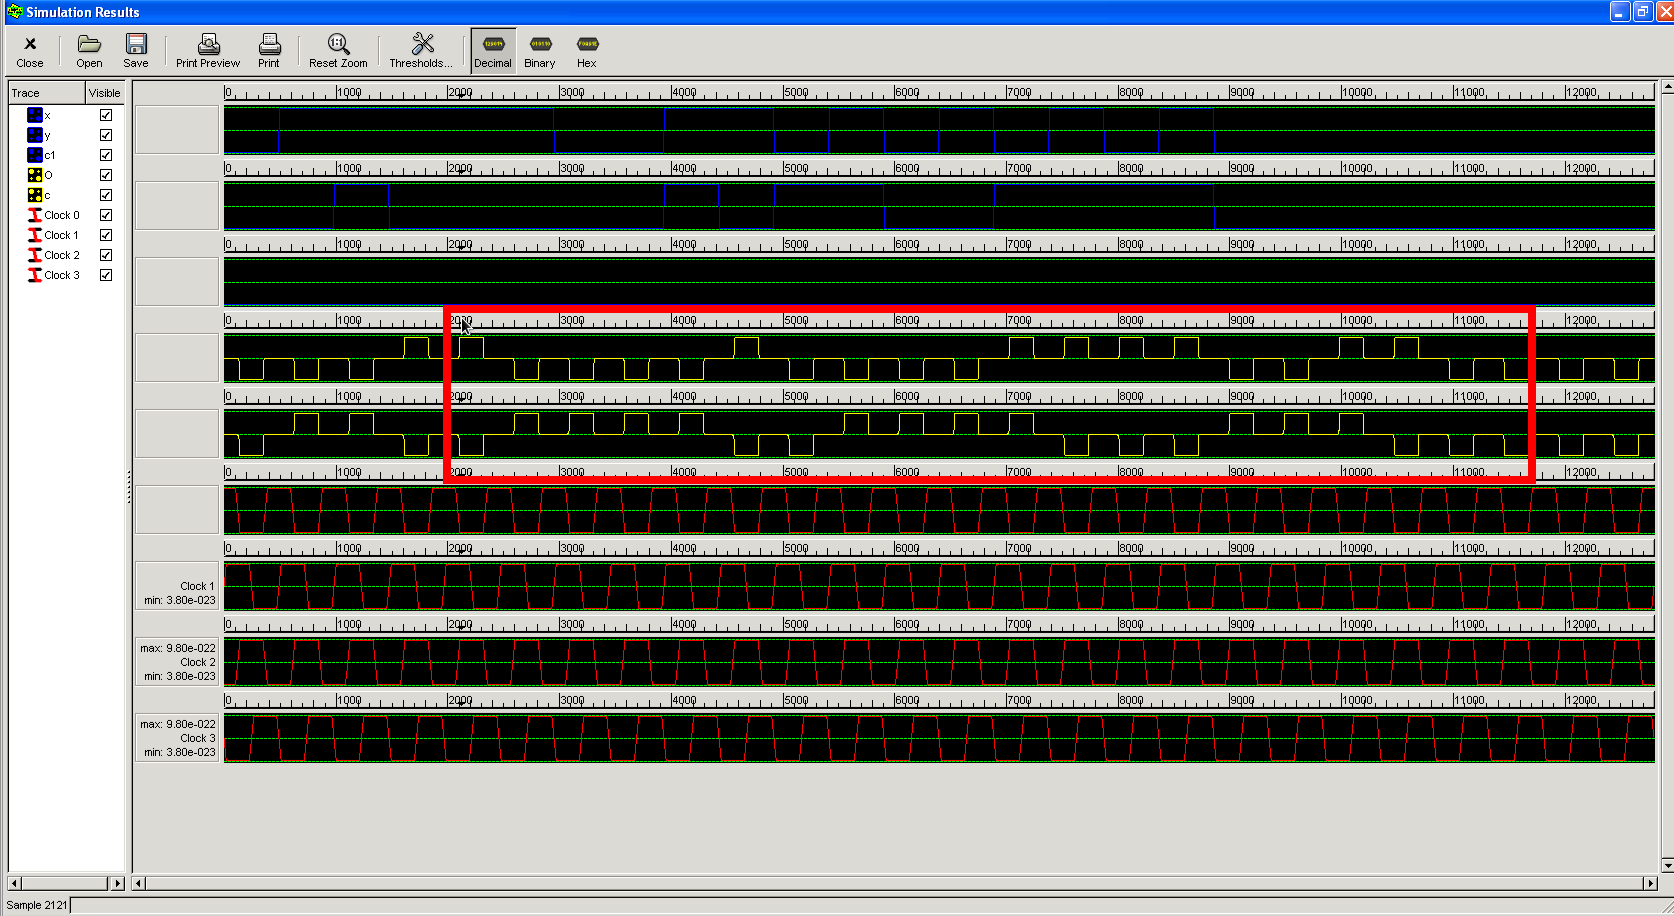
\includegraphics[width=14cm]{simulacije/long}
\caption{Seštevanje večjih števil}
\label{sestevalnik}
\end{figure}
\end{minipage}

\pagebreak
\subsection{Težave s QCAdesignerjem}
Pri delu s programom QCAdesigner smo na žalost naleteli na veliko težav.
\begin{itemize}
\item Zelo pogosto sesuvanje programa
\item Nedelovanje Linux verzije programa v Ubuntu 11.10
\item Naključno brisanje, zaklepanje in nedelovanje vektorske tabele pri simulaciji
\item Problem z decimalnimi vejicami oz. pikami pri shranjenih datotekah
\item Občasno precej naključni in popolnoma nepričakovani rezultati simulacij in to že pri preprostih vezjih
\end{itemize}

\begin{figure}[H]
\begin{center}
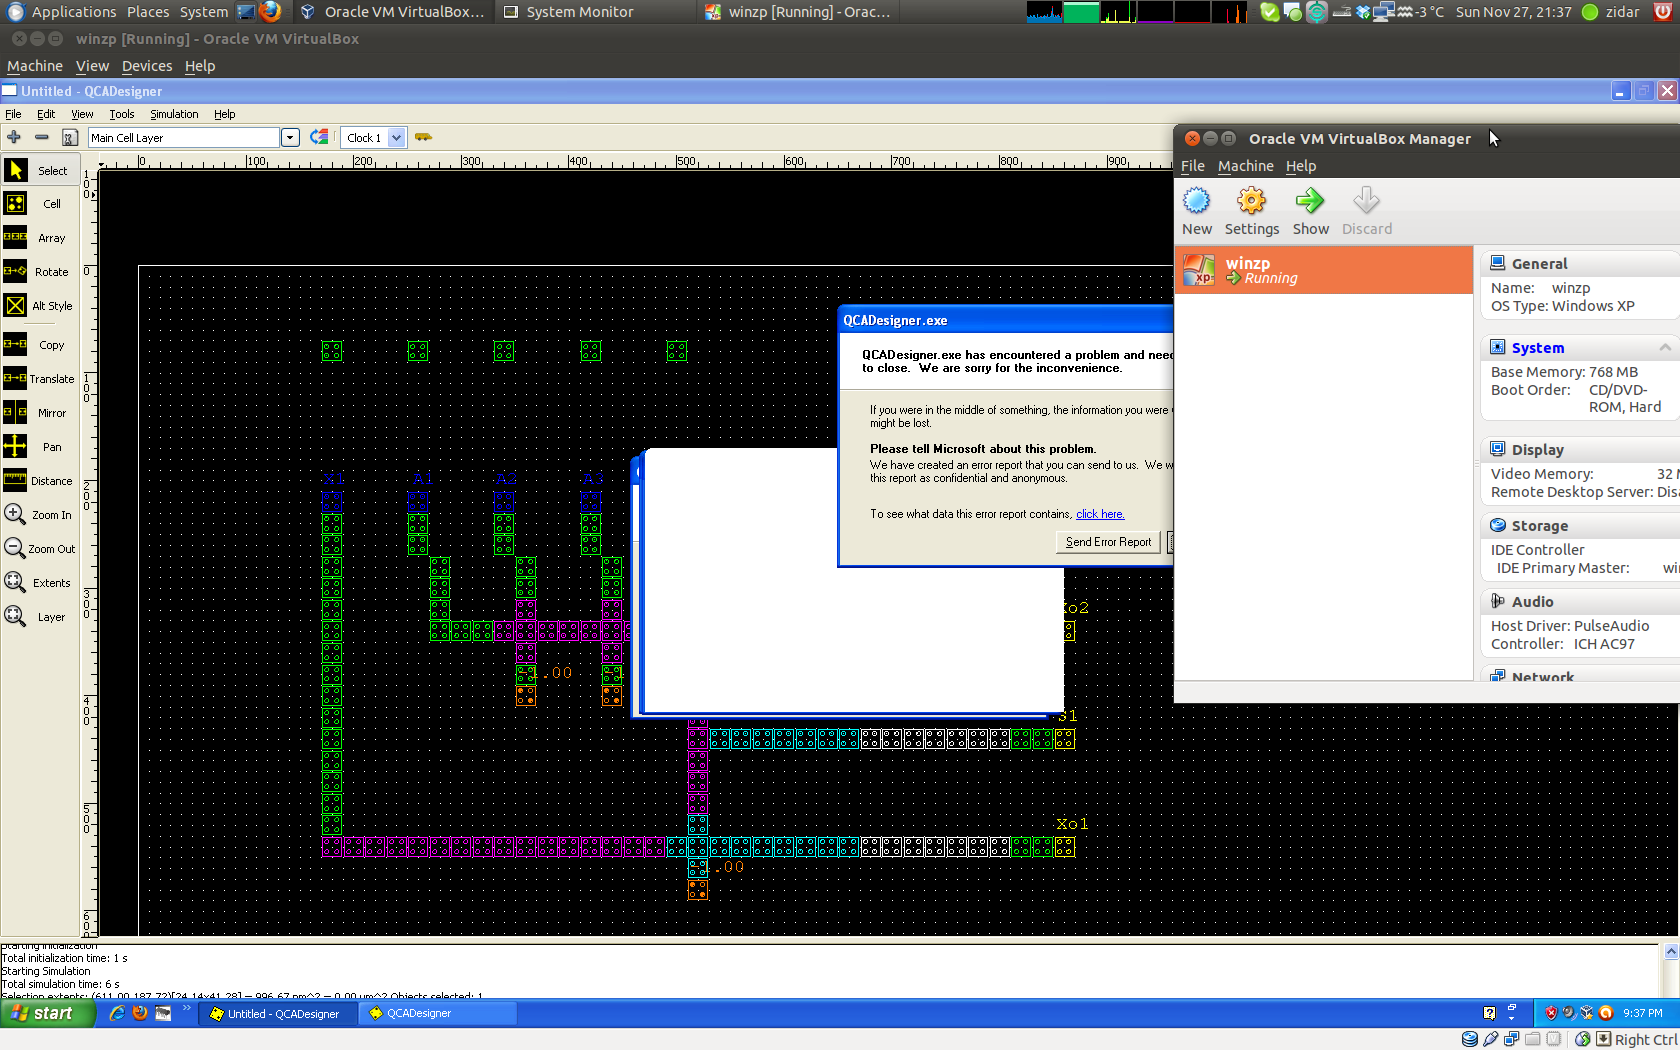
\includegraphics[width=14cm]{qca/img/screenshot}
\end{center}
\end{figure}

%
%%
\section{Zaključek}
Z veliko truda in precejšnjimi težavami s QCAdesigner-jem, nam je uspelo realizirati posamezne dele ALE, ni pa nam uspelo komponent sestaviti skupaj v delujočo ALE.

%
%%
\References
\bibliographystyle{elsart-num-sl}
\bibliography{sample}

\end{document}
